\documentclass[dvipdfmx]{jsarticle}
\usepackage[dvipdfmx]{graphicx}
\graphicspath{{ピクチャ/}}
\usepackage{otf}
\usepackage[dvipdfmx]{graphicx}
\usepackage{amsmath,amssymb}
\usepackage{url}
\begin{document}

\title{\huge 英語論文セミナー 第一回\\極限環境下における相関電子系中の磁場構造の測定}
\date{}
\maketitle

\begin{flushright}
\Large
2022/5/23\\
学籍番号:s0319007\\
氏名:上野智也\\
\end{flushright}

\section{要旨}

圧力は、超伝導や磁性などの強相関電子系における競合する基底状態の中で、(クリーン?)で連続的そして系統的な調整パラメータである。しかし、高圧装置に格納された試料へのアクセスが制限されているため、充分な感度を持つ磁場センサーは稀である。私たちは、ダイヤモンド窒素空孔中心を、極低温・高圧下での物質研究のための(空間分解ベクトル場センサー?)として利用した。
BaFe$_2$(As$0.59$P$0.41$)$_2$の単結晶をベンチマークとして、超伝導転移温度、マイスナー状態での局所磁場プロファイル、及び臨界磁場を抽出した。本研究で開発した方法は、様々な量子多体系を調査し、理解するための明確なツールを提供するものである。

\section{本文}

強相関電子系は、外部摂動に敏感な様々な相をサポートする。例えば超伝導転移温度$T_c$は、フェルミ準位における相互作用の強さと状態密度の両方に敏感であり(1)、これらは外部パラメータを変えることで調整することが可能である。さらに、超伝導体は、磁性的、構造的、電子的な秩序状態など、他の相と競合することがよく知られている(例えば(2-5))。したがって、材料系に適切なパラメータを与えることができるため、新しい相に到達するための主要な実験ツールとなる。

最も成功した調整パラメータのひとつが静水圧で、これは試料に追加の化学的不均一性を導入することなく電子構造と相互作用強度を変化させる。多くの系において、圧力は特定の量子状態に到達するための唯一の方法である。圧力は、競合する相を抑制することで、超伝導の安定化に影響力のある役割を担っている。例えば、重い電子系金属間化合物CePd$_2$Si$_2$では、圧力によって反強磁性状態が抑制され、超伝導転移温度$T_c$が28 kbarでピークをむかえる超伝導相が誘起される(2)。鉄系BaFe$_2$As$_2$でも同様に、スピン密度波の状態を抑制する圧力によって超伝導を引き起こすことができる(6)。最近では、LaH$_{10-\delta}$において200 GPaで250~260 Kという非常に高いTcを持つ超伝導状態が報告されている(7, 8)。これらの結果は、圧力が強力な調整パラメータであるという見方を補強するだけでなく、超高圧下での超伝導の微視的な詳細を研究する必要性を訴えている。

高圧を発生させるために、試料は試料よりも桁違いに大きな圧力容器に封入される。さらに、安定した圧力環境を確保するため、試料への電気的アクセスは厳しく制限される。極限条件下ではさらなる制約が課される。このような厳しい実験状況下では、適用できる検出方法はごくわずかである。

負電荷を帯びた窒素空孔(NV)センターは、スピン1基底状態を持つダイヤモンドの点欠陥である。電子スピン共鳴(ESR)スペクトルは、蛍光率がスピンに依存しているため、光学検出磁気共鳴(ODMR)法により測定することができる。これらのスペクトルから、マイクロテスラHz$^{-1/2}$の感度で磁場を導き出すことができる(9-13)ほか、電場、温度、機械的ひずみも導き出すことができる。[詳細な説明は(20)に記載] (14-19)。NVセンターは、60 GPaまでの圧力下で、電場の大きさと方向の両方を感知することができる(16, 21)。さらに、NVセンターはサイズが小さいため、当然ながら高い空間分解能が得られ、量子多体系の特徴を微視的に研究することが可能になる。 そこで、NVセンターの磁場センシング能力とモアッサナイトアンビルセルの光学的アクセス性を組み合わせ、高圧下における試料周辺の局所磁場配置を探ることに成功した。本研究では、II型超伝導体であるBaFe$_2$(As$_{0.59}$P$_{0.41}$)$_2$の超伝導に伴う反磁性を高圧下で直接観測し、このアプローチの可能性を実証・検証した。使用した試料は $x$ = 0.41 の単結晶 BaFe$_2$(As$_{1-x}$P$_x$)$_2$ で、これは(ultraclean family?) BaFe$_2$(As$_{1-x}$P$_x$)$_2$ の一部である (22) 。$x$ = 0.33でT$_c$は最大となり、量子臨界点の明確な証拠を示している(23, 24)。したがって、BaFe$_2$(As$_{1-x}$P$_x$)$_2$は、超伝導と量子臨界の間の相互作用を探るのに理想的なプラットフォームである。図 1A に圧力セル内部の分解図を、図 1B に試料と NV の中心基準枠の関係を拡大した図を示す。また、図1Bに試料近傍の写真と蛍光画像を示す。マイクロコイルを試料に近づけることで、NVセンターがある試料空間に効率よくマイクロ波電力を伝達することができる。蛍光像の輝点は、試料表面に散布されたダイヤモンド粒子に含まれるNVセンターによるもので、圧力伝達液と混合される。ダイヤモンド粒子の典型的な大きさ(1μm)は、感度をよくするために光学的分解能より小さく、渦格子定数a$_V$(20)より大きくなるように選ばれた。今回は、3つのダイヤモンド粒子を戦略的に選んだ。NV$_{C}$は試料の中央付近、NV$_{E}$は試料の端付近、NV$_{F}$は試料から遠く離れた場所にある。

弱い外部磁場中では、T>Tcの場合、試料は通常状態にあり、NVセンターが感じる磁場は外部磁場と同じである(図1C)。しかし、T$_c$以下に冷却すると、試料から磁場が追い出され、材料表面付近の磁場プロファイルが変化し、これを試料表面のNVセンターが感じることができるようになる。NV$_{C}$では有効磁場が大きく減少し、NV$_E$では有効磁場が大きく増加している(図1D)。超伝導体がTcを越えて温められると、超伝導に関連した反磁性応答がTcで消失する。さらに、II型超伝導体では、印加磁場が下部臨界磁場(Hc1)よりも高い場合、磁場が試料を通過し始め、渦糸状態となる。渦糸状態は上部臨界磁場(Hc2)以上で完全に破壊され、その時点で超伝導体は通常の状態に戻る。これらのフィールド内挙動はすべて、試料表面に設置されたNVセンターによってプロファイルすることができる。

\newpage

\begin{figure}[h]
\centering
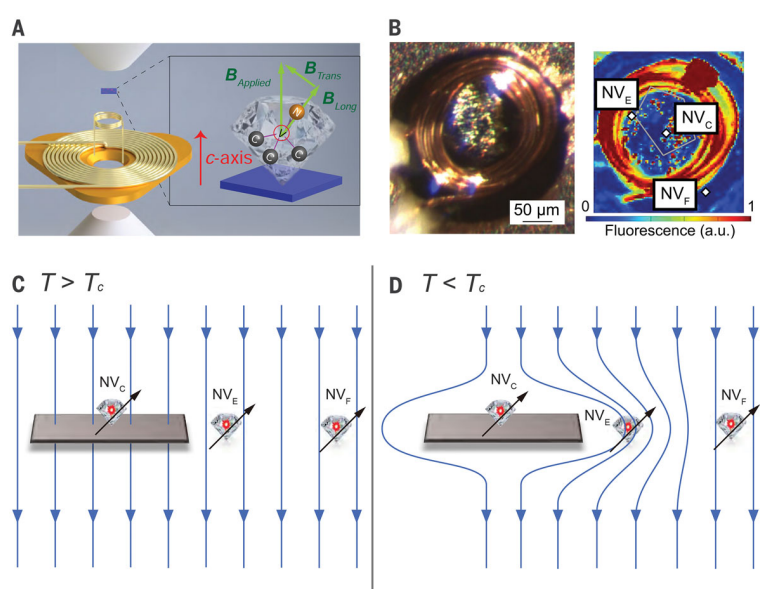
\includegraphics[width=12cm]{fig1.png}
\caption{実験構成と検出コンセプトの模式図}
\end{figure}%

図1のステートメント

(A) 圧力容器の分解図。試料(青色)は、ダイヤモンド粒子の集合体とともに高圧チャンバー内に配置されている。ダイヤモンド粒子の1つ1つが、高感度の局所磁場センサーである。レーザーは上部のモアッサナイトのアンビルを通して高圧室に向けて照射されます。マイクロ波は、試料に近接した小型マイクロコイルから供給されるため、試料を加熱することなく効率的にマイクロ波電力を伝達することができる。大きい方のコイルは、補助的な交流磁化率測定用の変調コイルとして追加される(26, 34)。モジュレーションコイルの下にある金属部分がガスケットである。拡大写真には、今回使用した2つの座標系が示されている。一つはc軸をFeAs面の積層方向とするサンプルフレーム、もう一つはNVセンターフレームである。本研究における外部印加磁場は、常に試料c軸に沿ったものである。ダイヤモンド粒子は、それぞれが4つの量子化軸を持つ約100万個のNV中心を含み、サンプルフレームに対してランダムに配向している(20)。

  

(B)(左)アンビルの上に試料を載せたマイクロコイルの写真。(右)マイクロコイルとNV中心を示す共焦点スキャンの蛍光画像。試料の形状を五角形でトレースしている。3つのダイヤモンド粒子、NV$_{C}$、NV$_{E}$、NV$_{F}$の位置が記されている。NV$_{C}$は上面の中央付近、NV$_{E}$は端部付近、NV$_{F}$は試料から遠く離れており、コントロールセンサーとして機能する。蛍光は650nmから800nmの間で収集される。

  

(CとD)(C) T>Tc、(D) T<Tcの場合、弱磁場印加時の試料周辺の磁場プロファイル。T$ < $Tcのときに磁場が消えるのは、超伝導に伴う反磁性によるものである。超伝導体の存在下で磁場プロファイルが変化することは、圧力下で完全な磁場ベクトルを空間分解能で測定する我々のセンサーの性能を実証するための理想的なプラットフォームとなる。

\newpage
\section{用語}
・相関電子系

物質中で電子間の相互作用(クーロン相互作用など)があるもの。相互作用が強いものを強相関電子系という。

  

・ダイヤモンド窒素空孔中心(別称NVC:Nitrogen vacancy center)

ダイヤモンド結晶中の複合欠陥の一種であり、不純物原子である窒素(Nitrogen)と空孔(Vacancy)が隣り合うことで形成される原子レベルの構造体。分裂した電子スピン準位を持ち、その利用により高感度な計測が可能となる。

  

・マイスナー状態

超伝導体が外部磁場を内部から排除している状態(完全反磁性)。

  

・摂動

平衡状態に対しての僅かな乱れ。

  

・静水圧

一様な重力の下に置かれた静止流体中の圧力。

  

・重い電子系

強相関系において電子はゆっくりと動くため、電子の質量が重くなったと解釈でき、重い電子系と呼ばれている。

  

・bar

圧力の単位。1 bar $= 10^5$ Pa

  

・スピン密度波

金属の各原子位置での磁気モーメントの大きさがサイン関数的に変調を受ける磁性のこと。

  

・電子スピン共鳴(ESR)

MRI:磁気共鳴画像診断(NMR:核磁気共鳴)の電子版。

    

・光検出磁気共鳴法(ODMR)

光学的に電子スピン共鳴(EPR)を検出する手法。EPRは電子スピン準位間をマイクロ波で共鳴させることにより不対電子を検出する手法であり、試料からの光を検出するものがODMRである。

\newpage


・モアッサナイト

炭化ケイ素SiCの鉱物。

  

・量子臨界点

絶対零度近傍において、磁場や圧力などの制御パラメータを変化させたとき、量子揺らぎによって秩序状態が壊されるパラメータの値を量子臨界点と呼ぶ。

  

・有効磁場

実際に感じる磁場。

  

・渦糸状態

第二種超伝導体において磁場が超電導体を部分的に貫いている状態。渦糸とは、細い磁場とその磁場が作り出す円(渦)電流を組み合わせたもの。







































\end{document}